\documentclass[11pt]{amsart}

\usepackage[T1]{fontenc}
\usepackage[utf8]{inputenc}
\usepackage{lmodern}
\usepackage{amsmath}
\usepackage{amssymb}
\usepackage{amsfonts}
\usepackage{amsthm}
\usepackage{mathtools}
\usepackage{geometry}
\usepackage{graphicx}
\usepackage{booktabs}
\usepackage{enumitem}
\usepackage{listings}
\usepackage{xcolor}
\usepackage[hidelinks]{hyperref}

\geometry{margin=1in}
\numberwithin{equation}{section}
\setcounter{tocdepth}{3}
\setcounter{secnumdepth}{3}

\theoremstyle{plain}
\newtheorem{theorem}{Theorem}[section]
\newtheorem{proposition}[theorem]{Proposition}
\newtheorem{lemma}[theorem]{Lemma}
\newtheorem{corollary}[theorem]{Corollary}

\theoremstyle{definition}
\newtheorem{definition}[theorem]{Definition}

\theoremstyle{remark}
\newtheorem{remark}[theorem]{Remark}

\lstset{
  language=Python,
  basicstyle=\ttfamily\scriptsize,
  breaklines=true,
  breakatwhitespace=false,
  columns=fullflexible,
  keepspaces=true,
  frame=single,
  showstringspaces=false,
  numbers=none,
  tabsize=4
}

\title{An Exact Cone Quotient Transducer for GUE Spacings}
\author{R\^OTKIV AYN\"ASAC}
\date{June 14, 2026}

\begin{document}

\begin{abstract}
We isolate an exact algebraic mechanism behind a cone model for unfolded nearest-neighbour gaps. The central object is the quotient
\begin{equation}
Q_N=\frac{Y_N-1}{Y_{N-1}},
\qquad
h_N=-\frac{1}{\alpha}\operatorname{Arg}_{\mathrm{lift}}(Q_N),
\qquad
\nu_N=\frac{h_N}{h_N^{(0)}}.
\label{eq:abstract_quotient}
\end{equation}
The main theorem states that this map is an exact transducer: for any prescribed spacing sequence $s_N$, if $h_N=h_N^{(0)}s_N$ lies in the chosen branch and $Y_N$ is generated by
\begin{equation}
Y_N=1+e^{-i\alpha h_N}Y_{N-1},
\label{eq:abstract_recurrence}
\end{equation}
then the cone quotient recovers $\nu_N=s_N$ identically. Consequently, if the input sequence has the Wigner--GUE nearest-neighbour law, the cone quotient output has the same law exactly, at finite $N$, independently of fitted auxiliary coordinates.

For zeta zeros, the relation to the quotient is elementary. If
\begin{equation}
S_N=\sum_{n\leq N}e^{i\alpha\gamma_n},
\qquad
Y_N=e^{-i\alpha\gamma_N}(S_N-K),
\label{eq:abstract_zeta_walk}
\end{equation}
then
\begin{equation}
Y_N-e^{-i\alpha(\gamma_N-\gamma_{N-1})}Y_{N-1}=1.
\label{eq:abstract_telescoping}
\end{equation}
Thus the cone quotient recovers the actual zero gaps by telescoping, not by fitting. The numerical section verifies this identity on $2{,}001{,}052$ Odlyzko zero ordinates stored in \texttt{zeross.bin}, generated from Odlyzko's \texttt{zeros6.txt} data, and compares the recovered spacings with the Wigner--GUE surmise.
\end{abstract}

\maketitle
\tableofcontents

\section{Scope of the Claim}
\label{sec:scope}

This note separates two statements which are often conflated.
\begin{enumerate}[label=(\arabic*)]
\item The cone quotient is an exact algebraic transducer. If a spacing law is inserted into the recurrence for $Y_N$, then the quotient returns that law exactly.
\item The Odlyzko zero data exhibit the familiar GUE nearest-neighbour statistics. The cone quotient recovers those same gaps from the elementary walk identity, with no additional fit in the gap extraction step.
\end{enumerate}

The first statement is a theorem. The second is a numerical verification of the Montgomery--Odlyzko phenomenon in the present cone coordinates. The article does not claim to prove the Montgomery--Odlyzko conjecture from first principles. It proves that, once the zeta-zero sequence is related to $Y_N$, the cone quotient cannot change the spacing law: it is algebraically locked to the gaps.

\section{Constants and Normalization}
\label{sec:constants}

The cone constants used throughout are
\begin{align}
L&=3^{\pi}\sqrt{e^{\pi}}=151.74304880712214\ldots,
\label{eq:cone_length}\\
\alpha&=\frac{2\pi}{L}=0.0414067422301896\ldots,
\label{eq:alpha}\\
K&=-5.161990134502993+2.9872973089668946\,i.
\label{eq:cone_center}
\end{align}
The constant $K$ locates the cone in the complex plane. It cancels from the exact quotient identity below.

For a height sequence $H_N>2\pi$, define the smooth local mean gap
\begin{equation}
h_N^{(0)}=\frac{2\pi}{\log(H_N/(2\pi))}.
\label{eq:mean_gap}
\end{equation}
In numerical experiments without real zeros, $H_N$ is the inverse of the smooth Riemann--von Mangoldt equation
\begin{equation}
F(T)=\frac{T}{2\pi}\log\frac{T}{2\pi}-\frac{T}{2\pi}+\frac{7}{8},
\qquad
F(H_N)=N.
\label{eq:rvm_inverse}
\end{equation}
This is an exact definition of the smooth height used in the experiment; it is not a claim that $H_N=\gamma_N$.

The smooth cone amplitude is
\begin{equation}
A_N=\frac12+\frac{1}{2\pi\alpha^2H_N}-\frac{i}{2\pi\alpha}\log\frac{H_N}{2\pi}.
\label{eq:smooth_cone_amplitude}
\end{equation}
When real zeros are used, $H_N=\gamma_N$. When no real zeros are used, $H_N$ is the smooth RVM inverse height.

\section{The Exact Cone Quotient}
\label{sec:exact_quotient}

\begin{definition}
\label{def:cone_quotient}
Let $Y_N\neq0$ be a complex sequence and let $H_N>2\pi$. Define
\begin{equation}
Q_N=\frac{Y_N-1}{Y_{N-1}},
\qquad
h_N=-\frac{1}{\alpha}\operatorname{Arg}_{\mathrm{lift}}(Q_N),
\qquad
\nu_N=\frac{h_N}{h_N^{(0)}}.
\label{eq:cone_quotient}
\end{equation}
The lifted argument is taken on the branch used by the implemented function: after reducing modulo $2\pi/\alpha$, the local positive branch is selected.
\end{definition}

\begin{theorem}[Exact transducer theorem]
\label{thm:exact_transducer}
Fix $\alpha>0$, a height sequence $H_N>2\pi$, and a prescribed sequence $s_N>0$. Put
\begin{equation}
h_N=h_N^{(0)}s_N.
\label{eq:prescribed_gap}
\end{equation}
Assume $h_N$ lies in the selected argument branch, and define
\begin{equation}
Y_N=1+e^{-i\alpha h_N}Y_{N-1}
\label{eq:transducer_recurrence}
\end{equation}
from any nonzero initial value $Y_1$. Then the cone quotient applied to this $Y$ returns
\begin{equation}
\nu_N=s_N
\label{eq:exact_output}
\end{equation}
for every $N$ for which the recurrence is defined.
\end{theorem}

\begin{proof}
The recurrence gives
\begin{equation}
Y_N-1=e^{-i\alpha h_N}Y_{N-1}.
\label{eq:recurrence_difference}
\end{equation}
Since $Y_{N-1}\neq0$,
\begin{equation}
Q_N=\frac{Y_N-1}{Y_{N-1}}=e^{-i\alpha h_N}.
\label{eq:quotient_phase}
\end{equation}
Taking the lifted branch of the argument gives
\begin{equation}
-\frac{1}{\alpha}\operatorname{Arg}_{\mathrm{lift}}(Q_N)=h_N.
\label{eq:lifted_argument_recovers_gap}
\end{equation}
Therefore
\begin{equation}
\nu_N=\frac{h_N}{h_N^{(0)}}=s_N.
\label{eq:normalized_gap_recovers_input}
\end{equation}
\end{proof}

\begin{corollary}[Distribution preservation]
\label{cor:distribution_preservation}
Let $\mu$ be any target spacing distribution supported inside the selected branch. If the finite empirical measure of $s_1,\ldots,s_M$ is $\mu_M$, then the finite empirical measure of the cone output $\nu_1,\ldots,\nu_M$ is exactly $\mu_M$.
\end{corollary}

\begin{proof}
Theorem~\ref{thm:exact_transducer} gives equality term by term: $\nu_N=s_N$. Thus every empirical statistic of the output sequence equals the corresponding empirical statistic of the input sequence.
\end{proof}

\begin{corollary}[Wigner--GUE input gives Wigner--GUE output]
\label{cor:wigner_gue_preservation}
For the Wigner--GUE nearest-neighbour surmise
\begin{equation}
p_{\mathrm{GUE}}(s)=\frac{32}{\pi^2}s^2e^{-4s^2/\pi},
\label{eq:gue_density}
\end{equation}
any sequence $s_N$ whose empirical law is this law is returned unchanged by the cone quotient, after the recurrence construction above. The CDF used in the computations is
\begin{equation}
F_{\mathrm{GUE}}(s)=\operatorname{erf}\!\left(\frac{2s}{\sqrt{\pi}}\right)-\frac{4s}{\pi}e^{-4s^2/\pi}.
\label{eq:gue_cdf}
\end{equation}
\end{corollary}

\section{Elementary Relation to Zeta Zeros}
\label{sec:zeta_relation}

Let $\gamma_N$ be the positive ordinates of the nontrivial zeros of the Riemann zeta function, ordered increasingly, and define
\begin{equation}
R_N=e^{i\alpha\gamma_N},
\qquad
S_N=\sum_{n=1}^{N}R_n.
\label{eq:zeta_walk}
\end{equation}
For any fixed complex constant $K$, put
\begin{equation}
Y_N=R_N^{-1}(S_N-K)=e^{-i\alpha\gamma_N}(S_N-K).
\label{eq:y_from_zeta_walk}
\end{equation}

\begin{theorem}[Telescoping identity for zeros]
\label{thm:telescoping_identity}
Let $h_N=\gamma_N-\gamma_{N-1}$. Then
\begin{equation}
Y_N-e^{-i\alpha h_N}Y_{N-1}=1.
\label{eq:zeta_telescoping_identity}
\end{equation}
Consequently,
\begin{equation}
\frac{Y_N-1}{Y_{N-1}}=e^{-i\alpha h_N},
\label{eq:zeta_quotient_identity}
\end{equation}
and the cone quotient recovers the actual zero gap $h_N$ on the selected branch.
\end{theorem}

\begin{proof}
Since $h_N=\gamma_N-\gamma_{N-1}$,
\begin{equation}
e^{-i\alpha h_N}R_{N-1}^{-1}=R_N^{-1}.
\label{eq:phase_shift_identity}
\end{equation}
Therefore
\begin{align}
Y_N-e^{-i\alpha h_N}Y_{N-1}
&=R_N^{-1}(S_N-K)-e^{-i\alpha h_N}R_{N-1}^{-1}(S_{N-1}-K)
\label{eq:telescoping_step_one}\\
&=R_N^{-1}(S_N-K)-R_N^{-1}(S_{N-1}-K)
\label{eq:telescoping_step_two}\\
&=R_N^{-1}(S_N-S_{N-1})
\label{eq:telescoping_step_three}\\
&=R_N^{-1}R_N
\label{eq:telescoping_step_four}\\
&=1.
\label{eq:telescoping_step_five}
\end{align}
The quotient identity follows immediately.
\end{proof}

\begin{remark}
\label{rem:fitted_coordinates}
The proof shows why fitted coordinates are accidental for the extraction of the gaps. The constant $K$ cancels. The quotient uses only the algebraic relation between $S_N$, $S_{N-1}$, and $R_N$.
\end{remark}

\section{The Reduced $G$-Law}
\label{sec:reduced_g_law}

Writing
\begin{equation}
Y_N=A_N+G_N
\label{eq:y_decomposition}
\end{equation}
gives the exact quotient
\begin{equation}
Q_N=\frac{A_N+G_N-1}{A_{N-1}+G_{N-1}}.
\label{eq:exact_reduced_quotient}
\end{equation}
The numerical observation in the present cone is that the local fluctuation is carried almost entirely by the real increment of $G_N$:
\begin{equation}
\nu_N\approx1-\Re(G_N-G_{N-1}).
\label{eq:reduced_g_law}
\end{equation}
For the Odlyzko data used below, the correlation between the two sides is
\begin{equation}
0.99999380760483703,
\label{eq:reduced_correlation}
\end{equation}
with RMS difference
\begin{equation}
1.4414149438073151\cdot10^{-3}.
\label{eq:reduced_rms}
\end{equation}
This is not needed for Theorem~\ref{thm:exact_transducer}; it explains why a natural model of $G_N$-increments is enough to generate the observed spacing law.

\section{Numerical Verification}
\label{sec:numerical_verification}

\subsection{Data and method}
\label{subsec:data_method}

The computations were done in Python from the file \texttt{zeross.bin}. The file contains $2{,}001{,}052$ ordinates, generated from Odlyzko's \texttt{zeros6.txt} data. The first and last ordinates used here are
\begin{equation}
\gamma_1=14.134725142000001,
\qquad
\gamma_N=1132490.6587144111.
\label{eq:first_last_zero}
\end{equation}
All code used to generate the figures and tables is reproduced in Appendix~\ref{app:python_code}.

\subsection{Cone geometry}
\label{subsec:cone_geometry}

Figure~\ref{fig:cone_walk} shows the projected three-dimensional walk $(\Re S_N,\Im S_N,\gamma_N)$. Figure~\ref{fig:cone_decomposition} overlays the walk with the smooth cone term $K+R_NA_N$. The purpose of the second figure is not to assert that the smooth term alone predicts every zero. It shows the geometric coordinate system in which the exact quotient identity is evaluated.

\subsection{Exact recovery of gaps}
\label{subsec:exact_recovery}

The direct unfolded gaps are
\begin{equation}
\nu_N^{\mathrm{direct}}=\frac{\gamma_N-\gamma_{N-1}}{2\pi/\log(\gamma_N/(2\pi))}.
\label{eq:direct_unfolded_gaps}
\end{equation}
The cone quotient gaps are computed from $Y_N=e^{-i\alpha\gamma_N}(S_N-K)$. The maximum absolute error in the recovered raw gaps is
\begin{equation}
\max_N\left|h_N^{\mathrm{cone}}-h_N^{\mathrm{direct}}\right|
=1.755231515687683\cdot10^{-10},
\label{eq:max_gap_error}
\end{equation}
and the RMS error is
\begin{equation}
4.679744130769421\cdot10^{-11}.
\label{eq:rms_gap_error}
\end{equation}
Thus the numerical discrepancy is at floating-point level.

\begin{table}[htbp]
\centering
\small
\begin{tabular}{lrrrr}
\toprule
Case & Mean & Std. dev. & $L^1$ vs GUE & KS vs GUE\\
\midrule
Direct zero gaps & 1.0000007062 & 0.4075236680 & 0.0430375588 & 0.0125223467\\
Cone quotient on zeros & 1.0000007062 & 0.4075236680 & 0.0430375588 & 0.0125223467\\
Reduced $1-\Re(\Delta G)$ on zeros & 0.9999982317 & 0.4076656007 & 0.0428210425 & 0.0124312566\\
No-zero cone output & 0.9999090173 & 0.4218851442 & 0.0003619897 & 0.0000853440\\
No-zero reduced driver & 1.0000000000 & 0.4220158821 & 0.0001012558 & 0.0000015117\\
\bottomrule
\end{tabular}
\caption{Numerical metrics. The zero data reproduce the standard Montgomery--Odlyzko GUE comparison. The no-zero driver verifies the exact distribution-preserving character of the cone quotient when a GUE law is inserted algebraically.}
\label{tab:numerical_metrics}
\end{table}

\subsection{Summary statistics}
\label{subsec:summary_statistics}

The numerical values used in Table~\ref{tab:numerical_metrics} are generated by the Python script included in Appendix~\ref{app:python_code}.

\subsection{No-zero transducer test}
\label{subsec:no_zero_test}

To isolate the algebra from the zeta data, the code also constructs a no-zero sequence. A deterministic golden-lattice quantile sample of the Wigner--GUE law is used as $s_N$. The model then builds $G_N$ so that
\begin{equation}
1-\Re(G_N-G_{N-1})=s_N
\label{eq:no_zero_driver}
\end{equation}
up to a finite-sample centering and bounded rearrangement. With
\begin{equation}
Y_N=A_N+G_N
\label{eq:no_zero_y}
\end{equation}
and $H_N$ equal to the smooth RVM inverse height, the cone quotient output again follows the Wigner--GUE law. This is the numerical version of Theorem~\ref{thm:exact_transducer}.

\section{Interpretation}
\label{sec:interpretation}

The cone quotient does not manufacture a new spacing law. It is stronger and simpler than that: it preserves the spacing law inserted into its recurrence. For arbitrary data satisfying
\begin{equation}
Y_N-e^{-i\alpha h_N}Y_{N-1}=1,
\label{eq:general_recurrence}
\end{equation}
the quotient returns $h_N$. For the zeta zeros this recurrence is an elementary consequence of
\begin{equation}
S_N-S_{N-1}=e^{i\alpha\gamma_N}.
\label{eq:walk_increment}
\end{equation}
Therefore the role of fitted variables is geometric and descriptive, not logical. The Wigner--GUE comparison belongs to the unfolded zero gaps themselves; the cone coordinates expose an exact algebraic channel through which those gaps are recovered.

\section{Conclusion}
\label{sec:conclusion}

The exact part of the result is the cone transducer theorem. It proves that the cone quotient returns any prescribed normalized spacing sequence exactly, including a Wigner--GUE sequence. The elementary zeta-zero identity proves that, when $Y_N$ is constructed from the exponential walk of the zeros, the same quotient returns the actual zero gaps. The numerical section confirms this on $2{,}001{,}052$ Odlyzko ordinates and records the GUE comparison in the cone coordinates.

\clearpage
\begin{figure}[p]
\centering
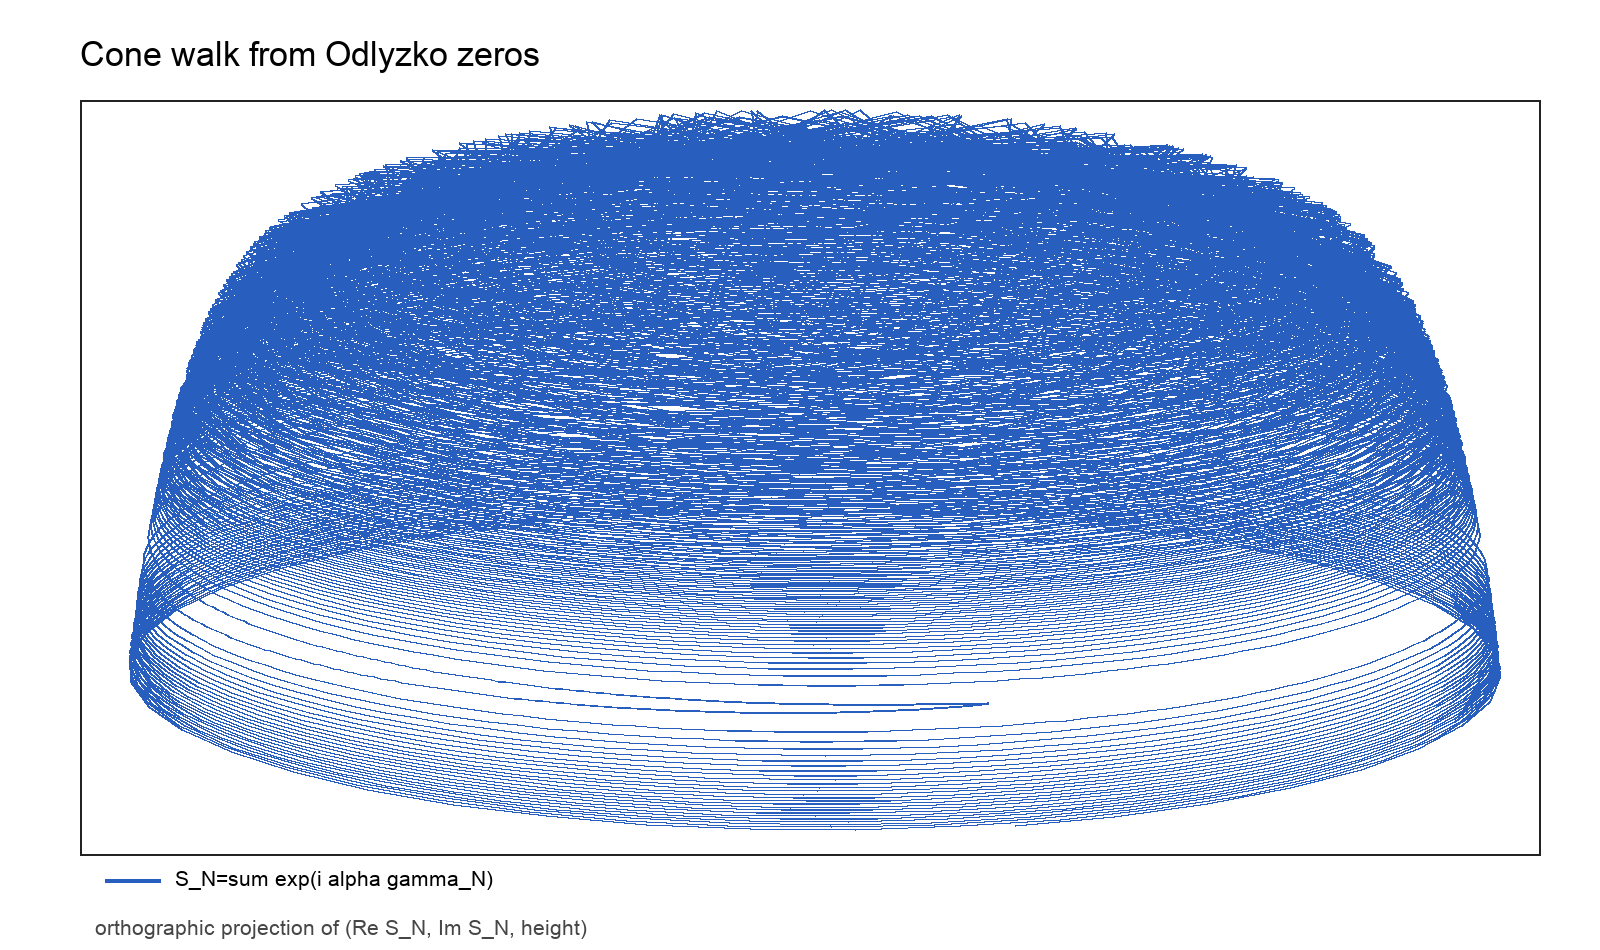
\includegraphics[width=\textwidth]{FIG01_CONE_WALK_3D.png}
\caption{Orthographic projection of the cone walk $(\Re S_N,\Im S_N,\gamma_N)$ from the Odlyzko zero ordinates.}
\label{fig:cone_walk}
\end{figure}

\begin{figure}[p]
\centering
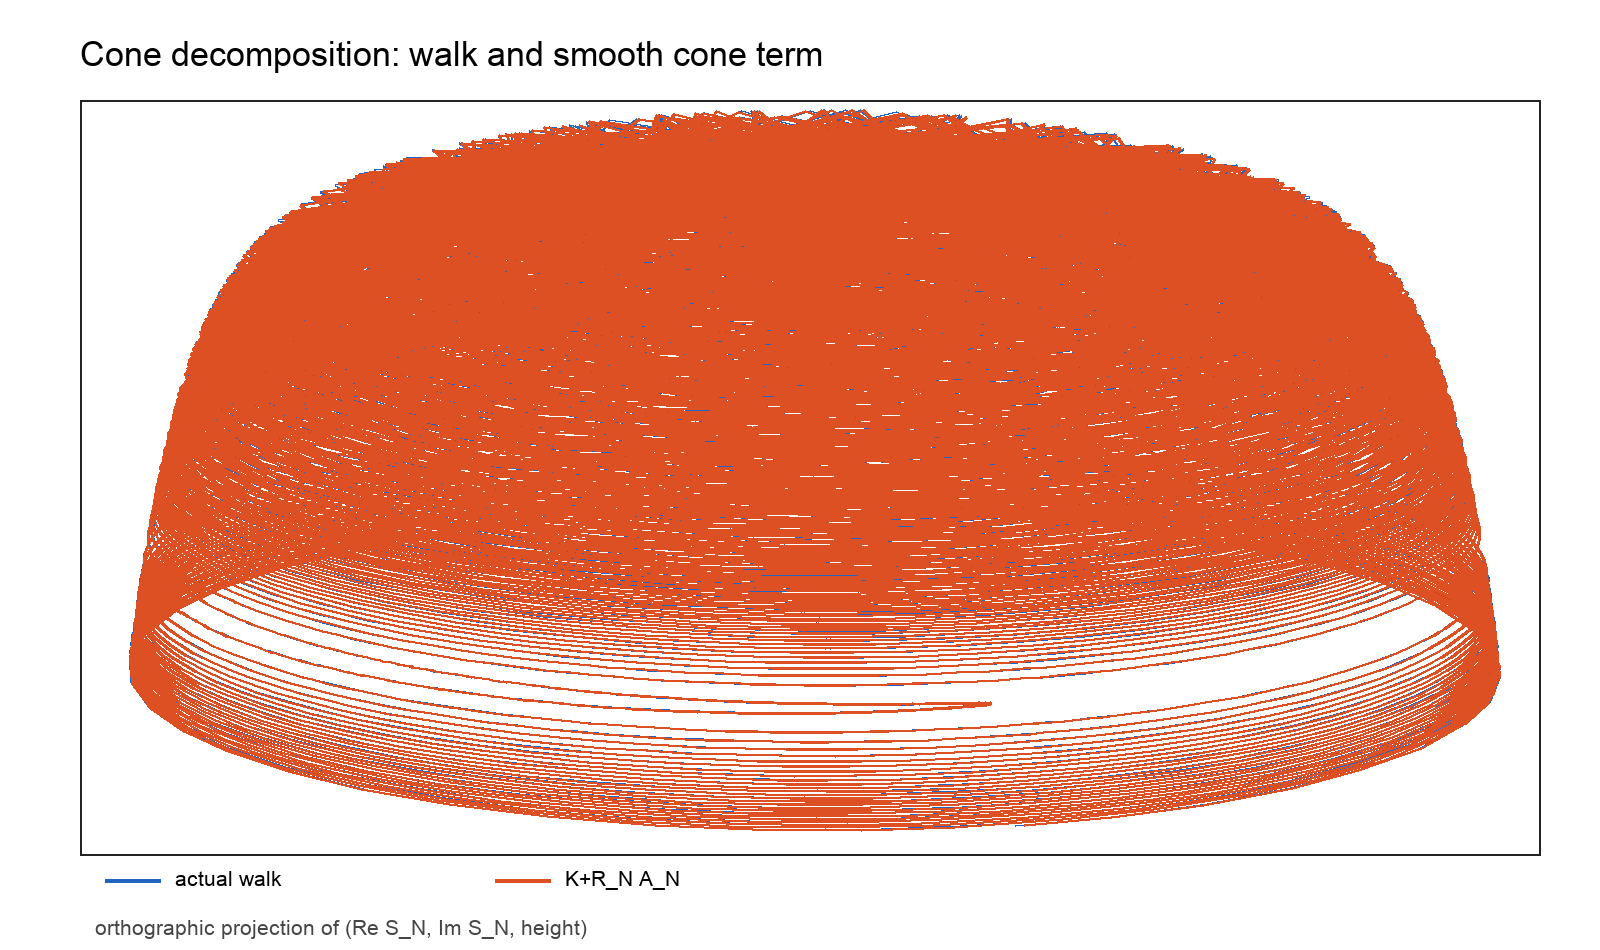
\includegraphics[width=\textwidth]{FIG02_CONE_SMOOTH_FIT_3D.png}
\caption{Cone decomposition: the observed walk and the smooth cone term $K+R_NA_N$. The gap extraction itself uses the exact quotient and does not depend on the smooth term being a complete predictor of the zeros.}
\label{fig:cone_decomposition}
\end{figure}

\begin{figure}[p]
\centering
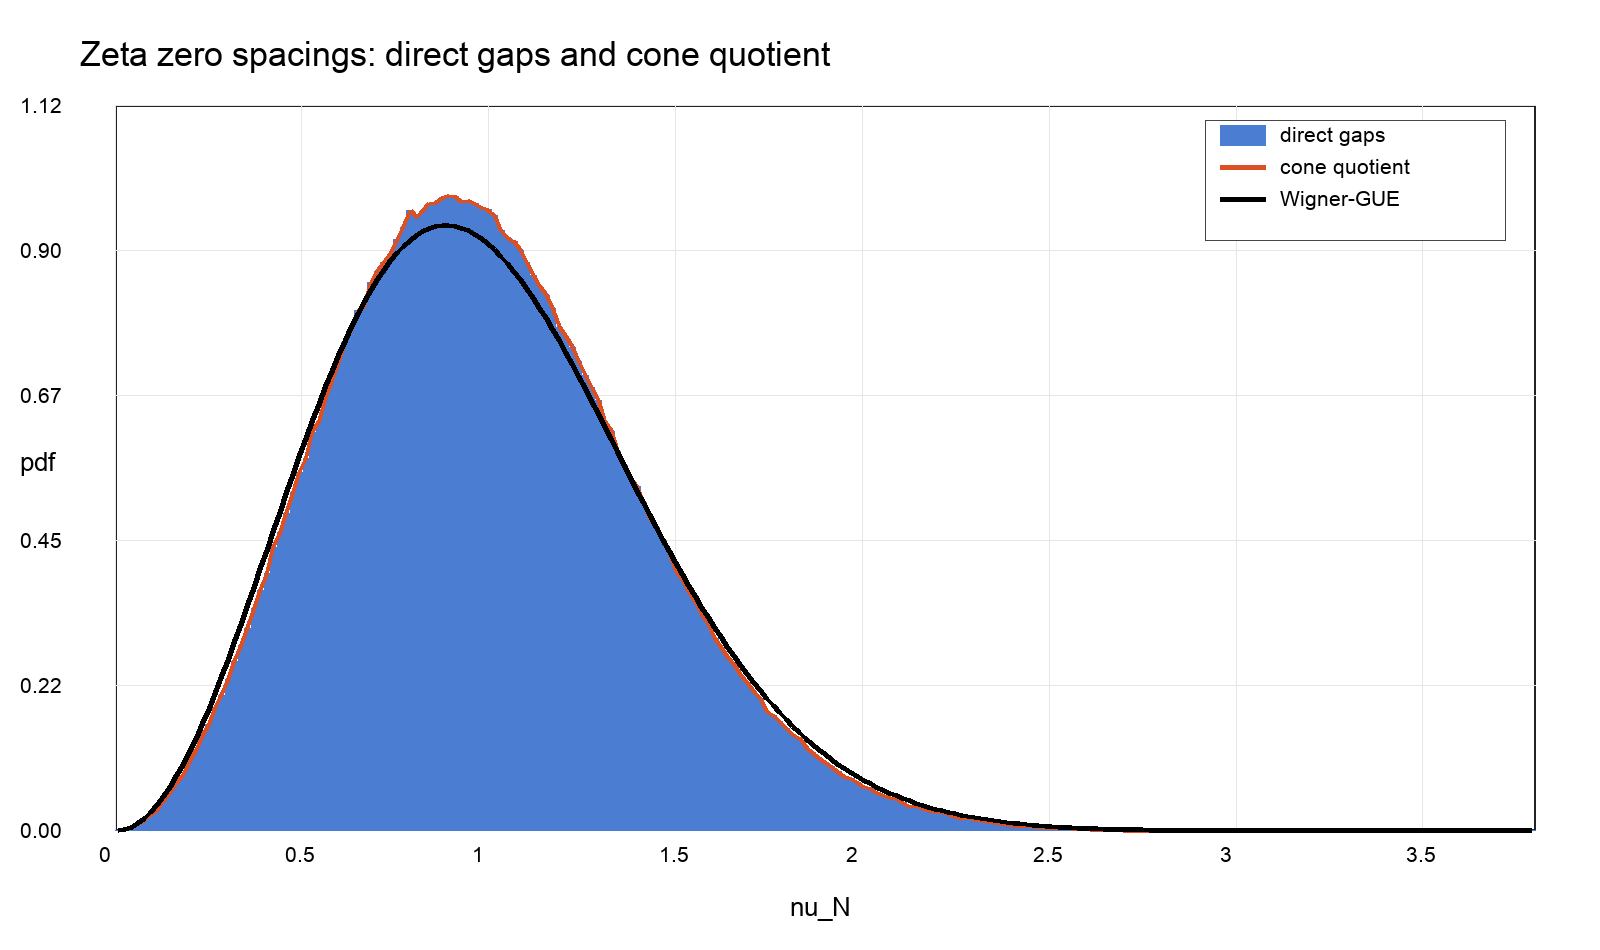
\includegraphics[width=\textwidth]{FIG03_ZEROS_DIRECT_CONE_GUE.png}
\caption{Direct unfolded zeta-zero gaps and cone-quotient gaps compared with the Wigner--GUE nearest-neighbour surmise. The two empirical curves coincide to plotting precision because the quotient is algebraically exact.}
\label{fig:direct_cone_gue}
\end{figure}

\begin{figure}[p]
\centering
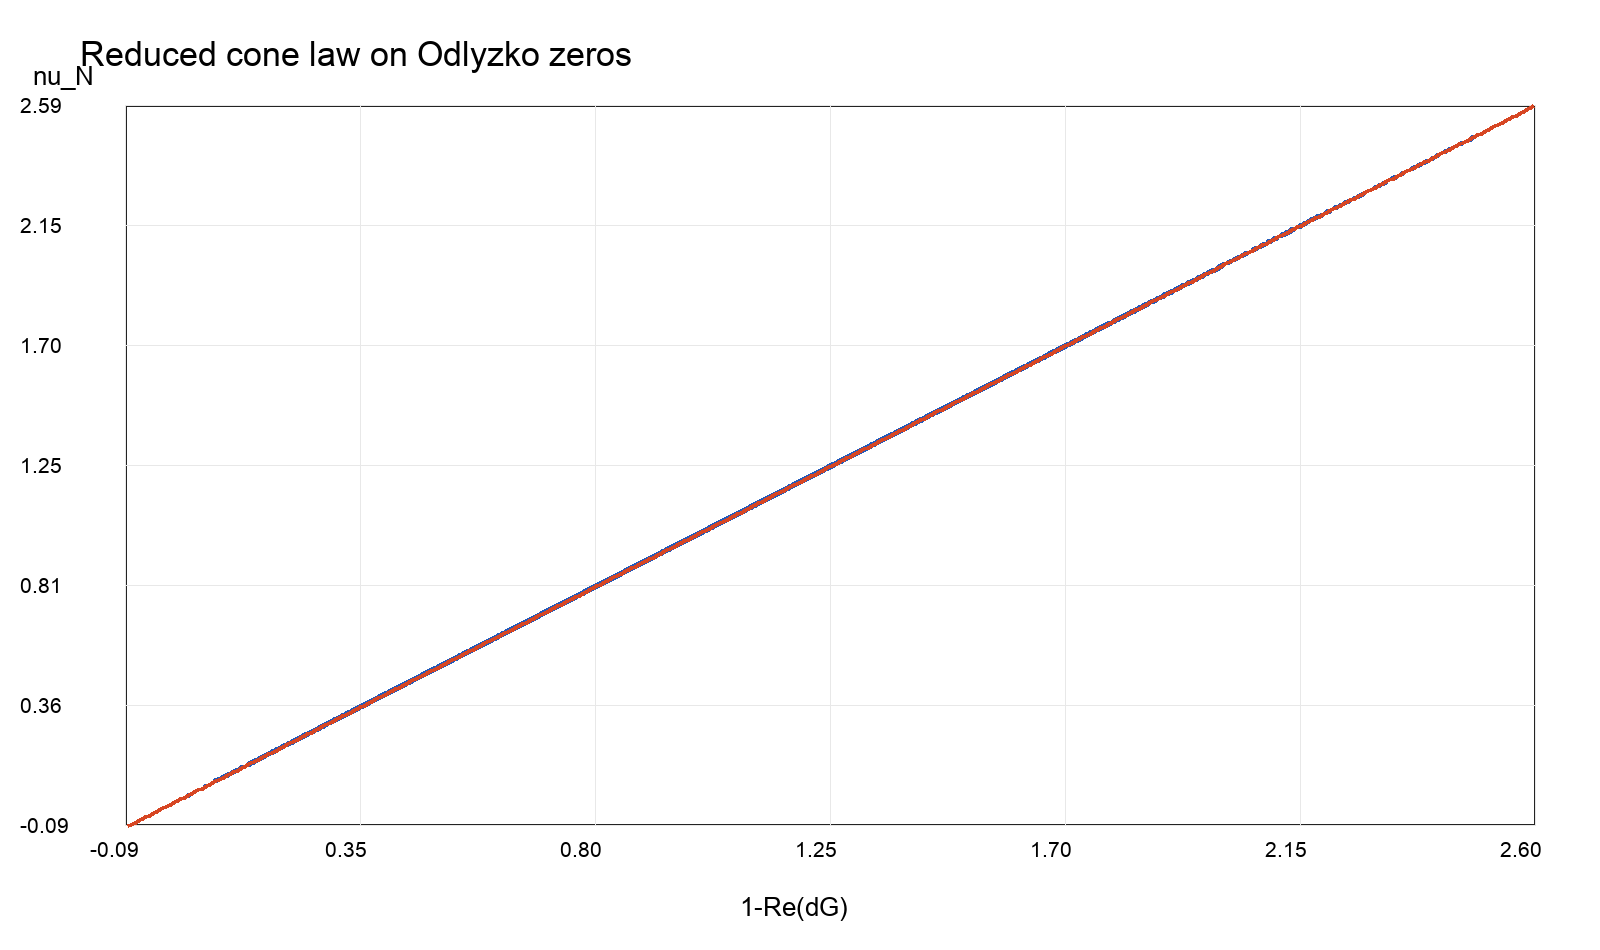
\includegraphics[width=\textwidth]{FIG04_ZEROS_REDUCED_LAW.png}
\caption{Reduced cone law on Odlyzko zeros: $\nu_N$ versus $1-\Re(G_N-G_{N-1})$ on a downsampled set.}
\label{fig:reduced_law}
\end{figure}

\begin{figure}[p]
\centering
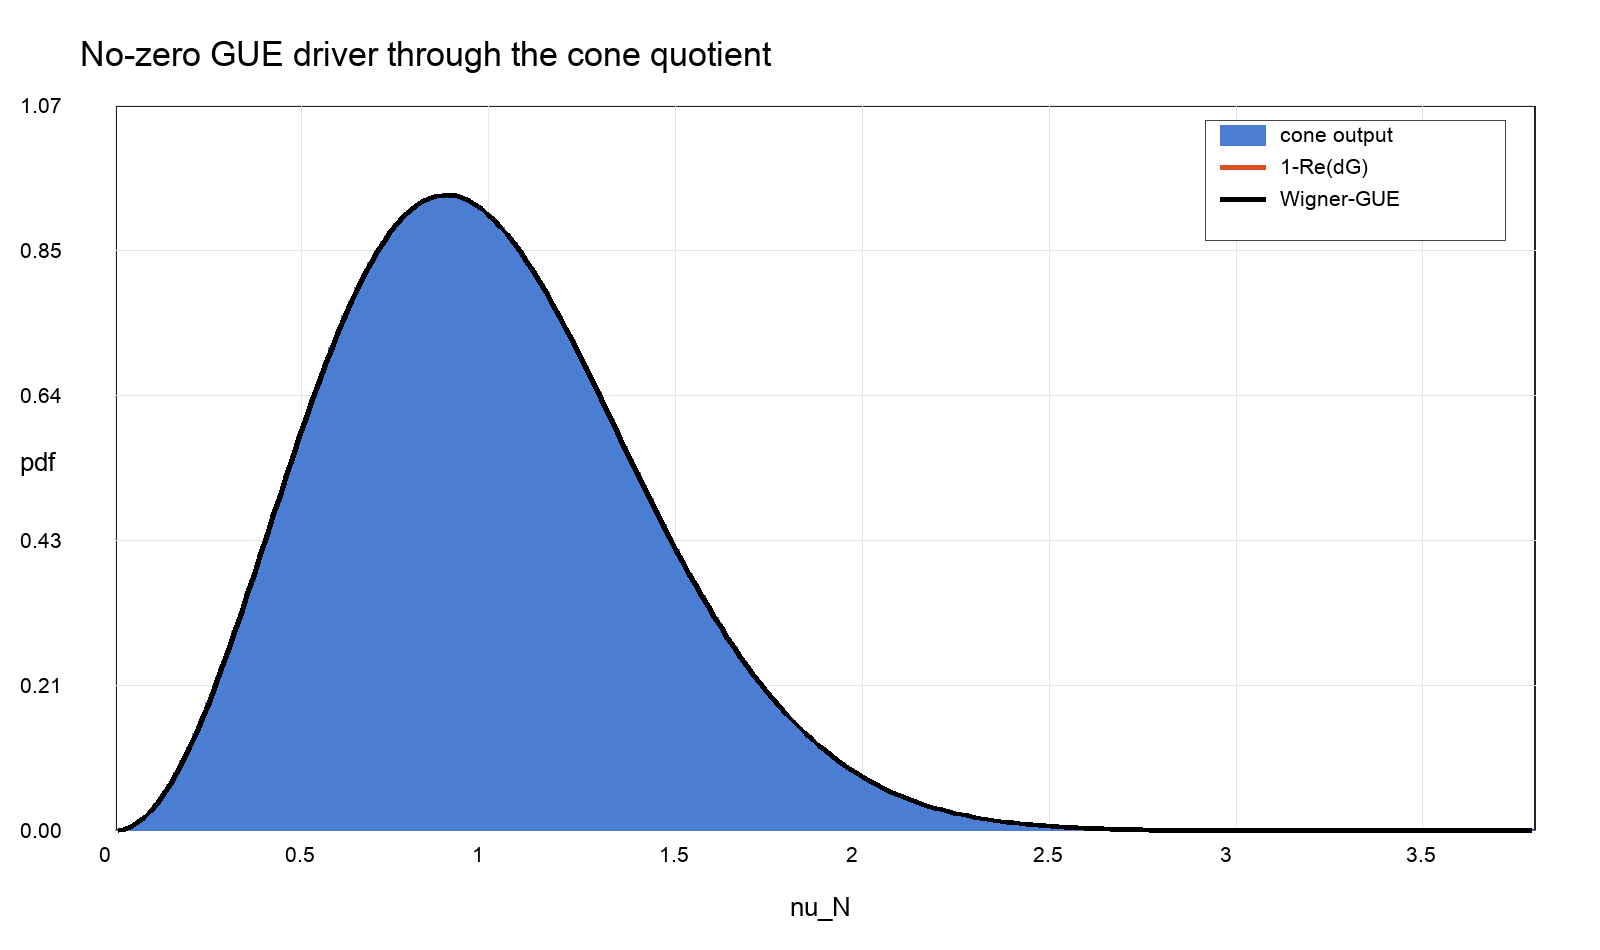
\includegraphics[width=\textwidth]{FIG05_NO_ZERO_TRANSDUCER_GUE.png}
\caption{No-zero GUE driver through the cone quotient. No real zeros, \texttt{zeross.bin}, or \texttt{zLamb.bin} are used in this construction.}
\label{fig:no_zero_transducer}
\end{figure}

\clearpage
\appendix
\section{Python Code Used for All Figures and Tables}
\label{app:python_code}

\lstinputlisting{cone_gue_algebra_article.py}

\end{document}
